
\subsection{CLU}
\label{sec:algorithms:clu}

\gls{clu}~\cite{Zhan2014} was first presented in 2014.
The authors of \gls{clu} recognize that recent research in \gls{llc} partitioning has followed two distinct directions.
Some publications optimize for access locality and attempt to improve performance by changing the lifetime of blocks in \gls{lru} managed caches.
\gls{dip}, \gls{tadip}, and \gls{nucache} are three such solutions that use novel methods to reduce or extend the lifetime of blocks in an elsewise \gls{lru} managed cache.
Other publications recognize the usefulness of utility and do way-partitioning between cores based on their utility values.
Examples here are \gls{ucp} and \gls{pipp}.
Both \gls{ucp} and \gls{pipp} are forced to use \gls{lru} as the underlying algorithm because they both depend on the stack property of \gls{lru} to do utility calculations~\cite{Qureshi2006, Xie2009}.

The authors of \gls{clu} present a novel approach for calculating the utility curve of a \gls{bip} managed cache.
\gls{bip}, as covered earlier, is one of the two insertion policies under \gls{dip} and \gls{tadip}. 
\gls{bip} violates the stack property of \gls{lru} by mostly inserting new rows at the \gls{mru} position, or at a low probability in \gls{lru} position.
To correctly measure the utility curve of a \gls{bip} managed k-way cache, one needs k \glspl{atd}; \gls{atd}($1$), \gls{atd}($2$), ... \gls{atd}($k$). 
Where \gls{atd}($x$) is an x-way \gls{atd}.
In contrast, the utility curve of an \gls{lru} managed cache can be found using one \gls{atd}, due to the stack property.
Having k \glspl{atd} per core sharing the \gls{llc} is not a realistic goal due to the required overhead.
The authors of \gls{clu} propose a simplification where there are $m = log_2 k$ \glspl{atd}; \gls{atd}($1$), \gls{atd}($2^1$), ..., \gls{atd}($2^m$).
A linear increase between the sample points is assumed when calculating the final utility curve.
It should be noted that the storage overhead of m \glspl{atd} in total is less than twice the overhead of the single \gls{atd}($k$) required to sample the \gls{lru} curve.

\gls{clu} uses the two curves first to allocate ways to each core using the same algorithm as shown for \gls{ucp} in Section~\ref{sec:algorithms:ucp}.
The only difference is that the algorithm uses either the \gls{lru} or \gls{bip} value when estimating utility given an allocation, depending on which algorithm performs best.
During runtime, \gls{clu} works like \gls{ucp}.
The only exception is that the core's ways are managed by either \gls{lru} or \gls{bip}, depending on which algorithm has the best utility value for the number of ways currently assigned to that core.

Figure~\ref{fig:algorithms:clu_example} is an example \gls{lip} and \gls{bip} utility plot for a core sharing a 16-way cache.
For each way value, the maximum achievable utility is the maximum of the \gls{lip} and \gls{bip} line.
Hence, when the lookahead algorithm is used to assign ways to each core, the maximum of the \gls{lip} and \gls{bip} value is used.
If the sample core were assigned 2 ways it would use \gls{bip} replacement, this follows from the fact that \gls{bip} has a higher utility at 2 ways.
However, if the core were assigned 12 ways, it would use \gls{lip} replacement because \gls{lip} has a higher utility at that point.

\begin{figure}[th]
    \centering
    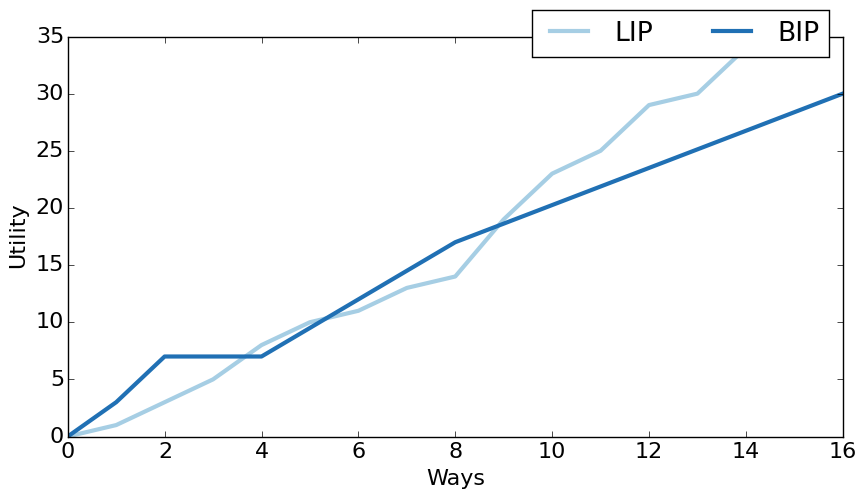
\includegraphics[width=.65\textwidth]{figures/algorithms/clu-utility}
    \caption{\gls{bip} and \gls{lip} utility plot in a 16-way cache.}
    \label{fig:algorithms:clu_example}
\end{figure}
